\section{Impulse, Momentum, and Interactions\footnote{
1990-93 Dept. of Physics and Astronomy, Dickinson College. Supported by FIPSE
(U.S. Dept. of Ed.) and NSF. Portions of this material may have been modified
locally and may not have been classroom tested at Dickinson College.
}}
\instructornote{%
This lab was slightly modified in Fall 2021 by Matt Trawick.

The previous version had sudents use an inclined track, having the cart accelerate towards the force probe.  My students seemed to find this confusing; they were trying to calculate the change in momentum from the top of the ramp to the bottom, rather than before and after the collision.

I've also added a data table, and tidied up various things.

By Will Hodge, fall 2023.  Updated to use wireless smart cart.
}

\makelabheader %(Space for student name, etc., defined in master.tex or labmanual_formatting_commands.tex)

\medskip
\textbf{Objectives }

\begin{itemize}[nosep]
\item To verify the relationship between impulse and momentum experimentally. 
\item To study the forces between objects that undergo collisions and other types of interactions in a short time period.
\end{itemize}

\medskip
\textbf{Apparatus} 
\begin{itemize}[nosep]
\item \textit{Capstone} software (\filename{Impulse-Momentum.cap} experiment file)
\item CS2000 compact scale
\item Dynamics track with track ends
\item Wireless smart cart with spring 
\end{itemize}
\textbf{The Impulse-Momentum Theorem }

Real collisions, like those between eggs and hands, a tennis ball and a wall, or
a falling ball and a table top are tricky to study because $\Delta t$ 
is so small and
the collision forces are not really constant over the time the colliding objects
are in contact. Thus, we cannot calculate the impulse as $F \,\Delta t$. 
Before we study
more realistic collision processes, let's redo the theory for a variable force.
In a collision, according to Newton's second law, the force exerted on a falling
ball by the table top at any infinitesimally small instant in time is given
by
\begin{equation}
{\vec  F}=\frac{d{\vec  p}}{dt}
\end{equation}

To describe a general collision that takes place between an initial time $t_{i}$
and a final time $t_{f}$ , we must take the integral of both sides of the
equation with respect to time. This gives

\begin{equation}
\int _{t_{i}}^{t_{f}}{\vec  F}dt=\int _{t_{i}}^{t_{f}}\frac{d{\vec  p}}{dt}dt=\left( {{\vec  p}_{f}}-{{\vec  p}_{i}}\right) =\Delta {\vec  p}.
\end{equation}

Impulse ${\vec  J}$ is a vector quantity defined by the equation
\begin{equation}
{\vec  J}=\int_{t_{i}}^{t_{f}}{\vec  F}\,dt,
\end{equation}
which represents the area under the $F$ \textit{vs.}\ $t$ 
curve.
By combining equations (2) and (3) we can formulate the impulse-momentum
theorem in which
\begin{equation}
{\vec  J}=\Delta {\vec  p}.
\end{equation}

\pagebreak
\textbf{Activity 1: Predicting Collision Forces That Change }

Let's see qualitatively what an impulse curve might look like in a real collision
in which the forces change over time during the collision. In particular, let's
consider the collision of a tennis ball with a wall as shown below.

\vspace{0.3cm}
%{\par\centering 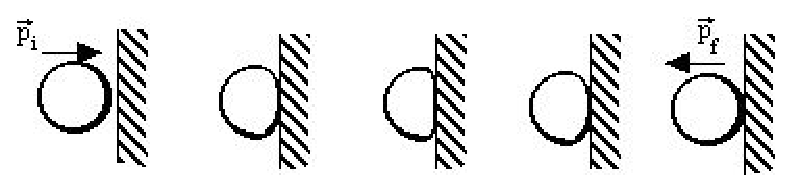
\includegraphics{impulse/impulse_fig1.eps} \par}
{\par\centering 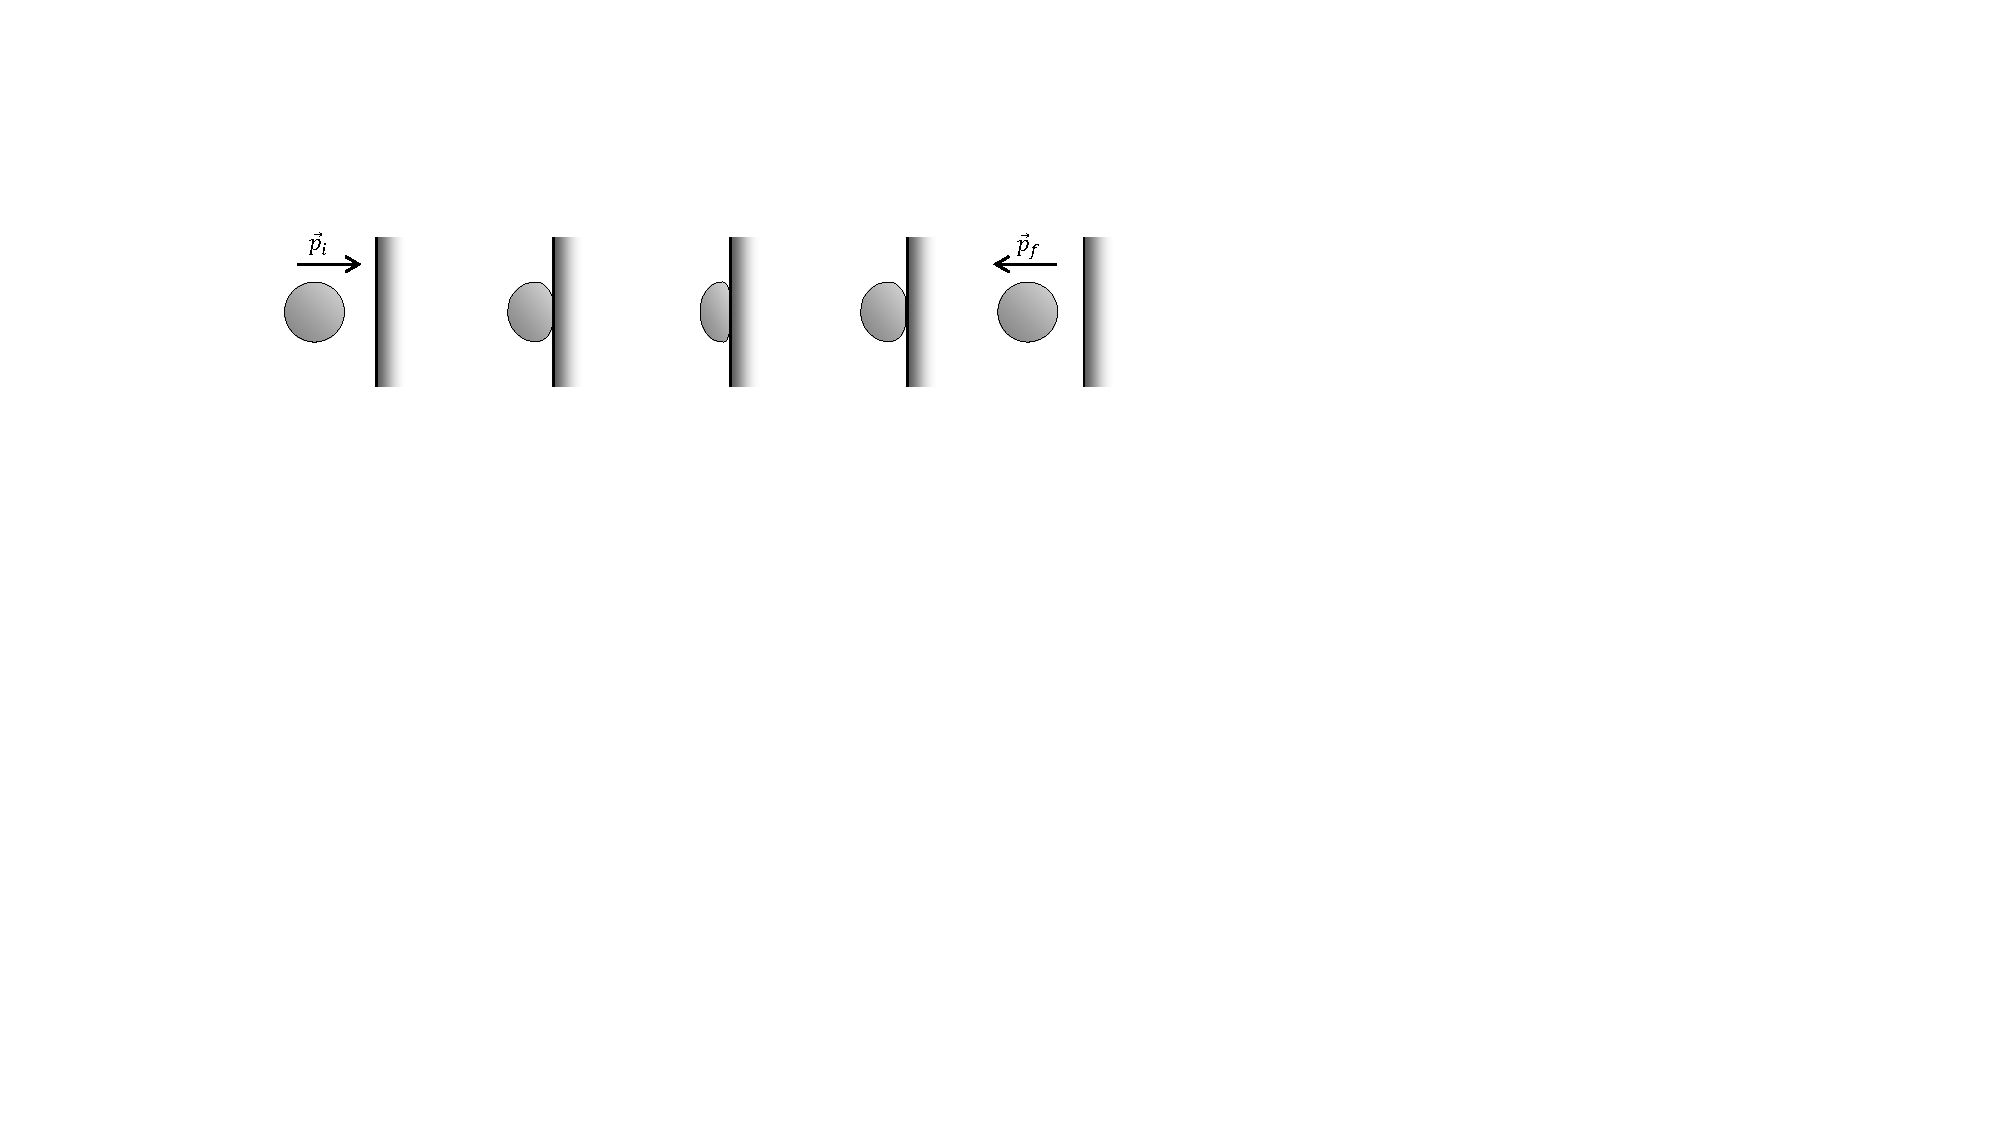
\includegraphics{impulse/ball_hitting_wall.pdf} \par}
\vspace{0.3cm}

(a) Suppose a tennis ball is barreling toward a wall and collides with it. If gravity and air friction are neglected, what is the net force exerted on the object just before it starts to collide?
\vspace{10mm}

(b) When will the magnitude of the force on the ball be a maximum? 
\vspace{10mm}

(c) Roughly how long does the collision process take? Half a second? Less? Several
seconds?
\vspace{10mm}

(d) Attempt a rough sketch of the shape of the force the wall exerts on a moving
object during a collision.

%\vspace{0.3cm}
%{\par\centering 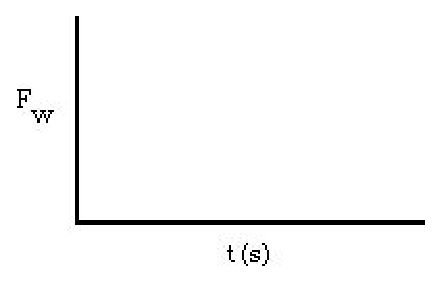
\includegraphics{impulse/impulse_fig2.eps} \par}
%\vspace{0.3cm}
\begin{lab_axis}*[lab_noticks_1quad,
	width=2in, height=1.4in,
	xlabel=Time,
	ylabel= {Force $F_{\rm wall}$}
]
\end{lab_axis}


\textbf{Activity 2: Verification of the Impulse-Momentum Theorem} 

To verify the impulse-momentum theorem experimentally we will show that for
an actual collision involving a single force on an object, the equation
\[
\int_{t_{i}}^{t_{f}}{\vec  F}\,dt=\Delta {\vec  p}\]


holds, where the impulse integral can be calculated by finding the area under
the curve of a graph of $F$ \textit{vs.}~$t$.

%\vspace{0.3cm}
%{\par\centering 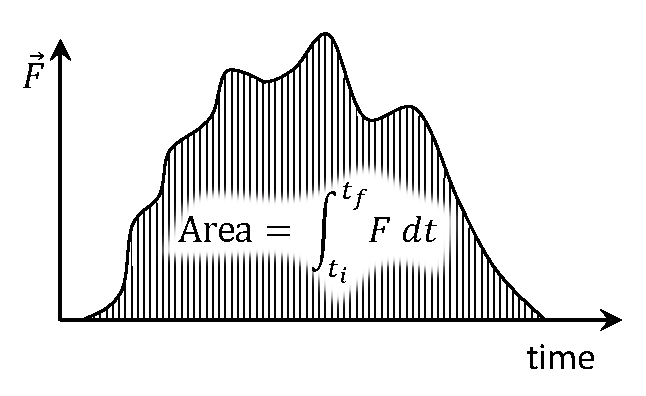
\includegraphics[width=2.5in]{impulse/impulse_fig3_new.eps} \par}
%\vspace{0.3cm}
\begin{lab_axis}*[lab_noticks_1quad,
	width=2.5in, height=1.2in,
	algebraic_labels,
	xlabel=$t$,
	ylabel= $F$,
	xmin=0,xmax=21,
	ymin=0,ymax=10,
]
\addplot +[smooth, tension=0.90, fill= lightgray] coordinates{(0,0) (1,0.5)(3,4) (6,5) (9,8)(11,9)(14,8)(18,1.5)(20,0)};
\addplot +[line width=0.8pt] coordinates{(0,0) (21,0)}; %fixes annoying problem that the fill partially paints over the axis
\node[anchor=south] at (axis cs: 10,0.5)  {Area $\displaystyle =\int_{t_{i}}^{t_{f}}{\vec  F}\,dt$};
\end{lab_axis}



The experimental setup is shown in the figure below.
%but with the force probe facing the open end of the track so it can be calibrated.  
Open the file \filename{Impulse-Momentum.cap} in the \filename{\coursefolder} folder. Turn on the cart at your station and connect it to the computer via Bluetooth. To tare the cart's built-in sensors, select the desired sensor (either the \textbf{Smart Cart Acceleration Sensor} or the \textbf{Smart Cart Force Sensor}) in the \textbf{Controls} palette and then click \textbf{Zero Sensor Now}. When taring the sensors, the cart should be at rest and there should be no applied force on the spring. 
 
%Calibrate the force probe 
%(see \textit{Calibrating Force Sensors} in \textbf{Appendix \ref{capstone}: Capstone}). 
%Remove pulley from end of track. Once calibrated, remove the force probe and 
%bracket by loosening wing bolts just enough to slide the entire assembly out the 
%end of the track. Reverse the assembly and slide the nuts in the slot on the 
%other side of the track and tighten wing bolts. Remove hook from force probe and 
%replace with light duty collision spring. The setup should now look like the figure 
%The setup should look like the figure below.
%Set the data acquisition rate 
%on the {\it Capstone} window to 100 Hz and tare the force sensor.
%With the track horizontal, give the cart a gentle shove towards the force probe.  (Be sure to %pull your hand away from the track afterwards so you can get a clean measurement of the cart's %velocity both before and after the collision with the probe.)
%The force probe will measure the force as a function of time during the collision. 
%The motion detector is used to measure the velocity of the cart before and after the 
%collision. You will use the Impulse-Momentum application to make these measurements.

\vspace{0.3cm}
%{\par\centering \resizebox*{0.9\textwidth}{!}{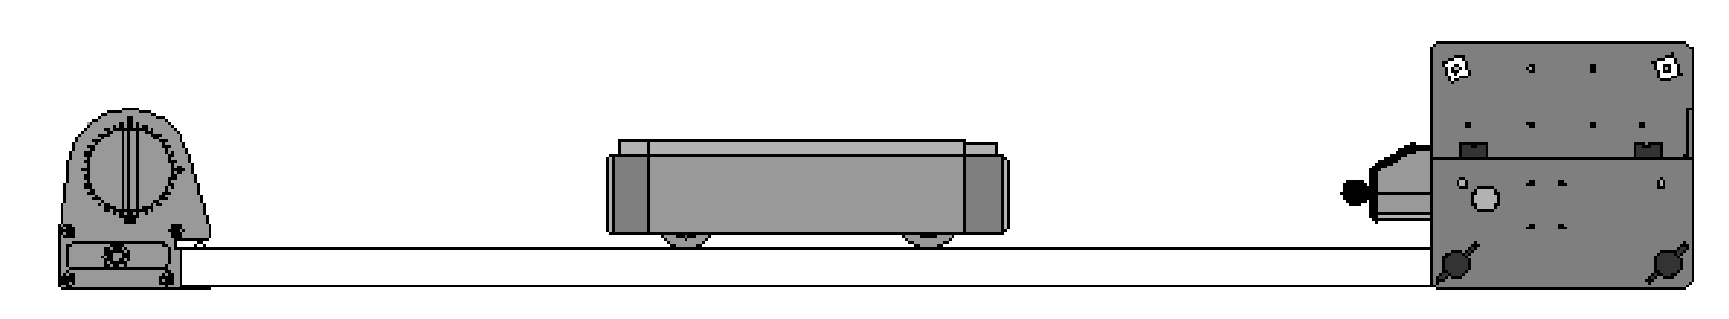
\includegraphics{impulse/impulse_fig4.eps}} \par}
%{\par\centering \resizebox*{0.9\textwidth}{!}{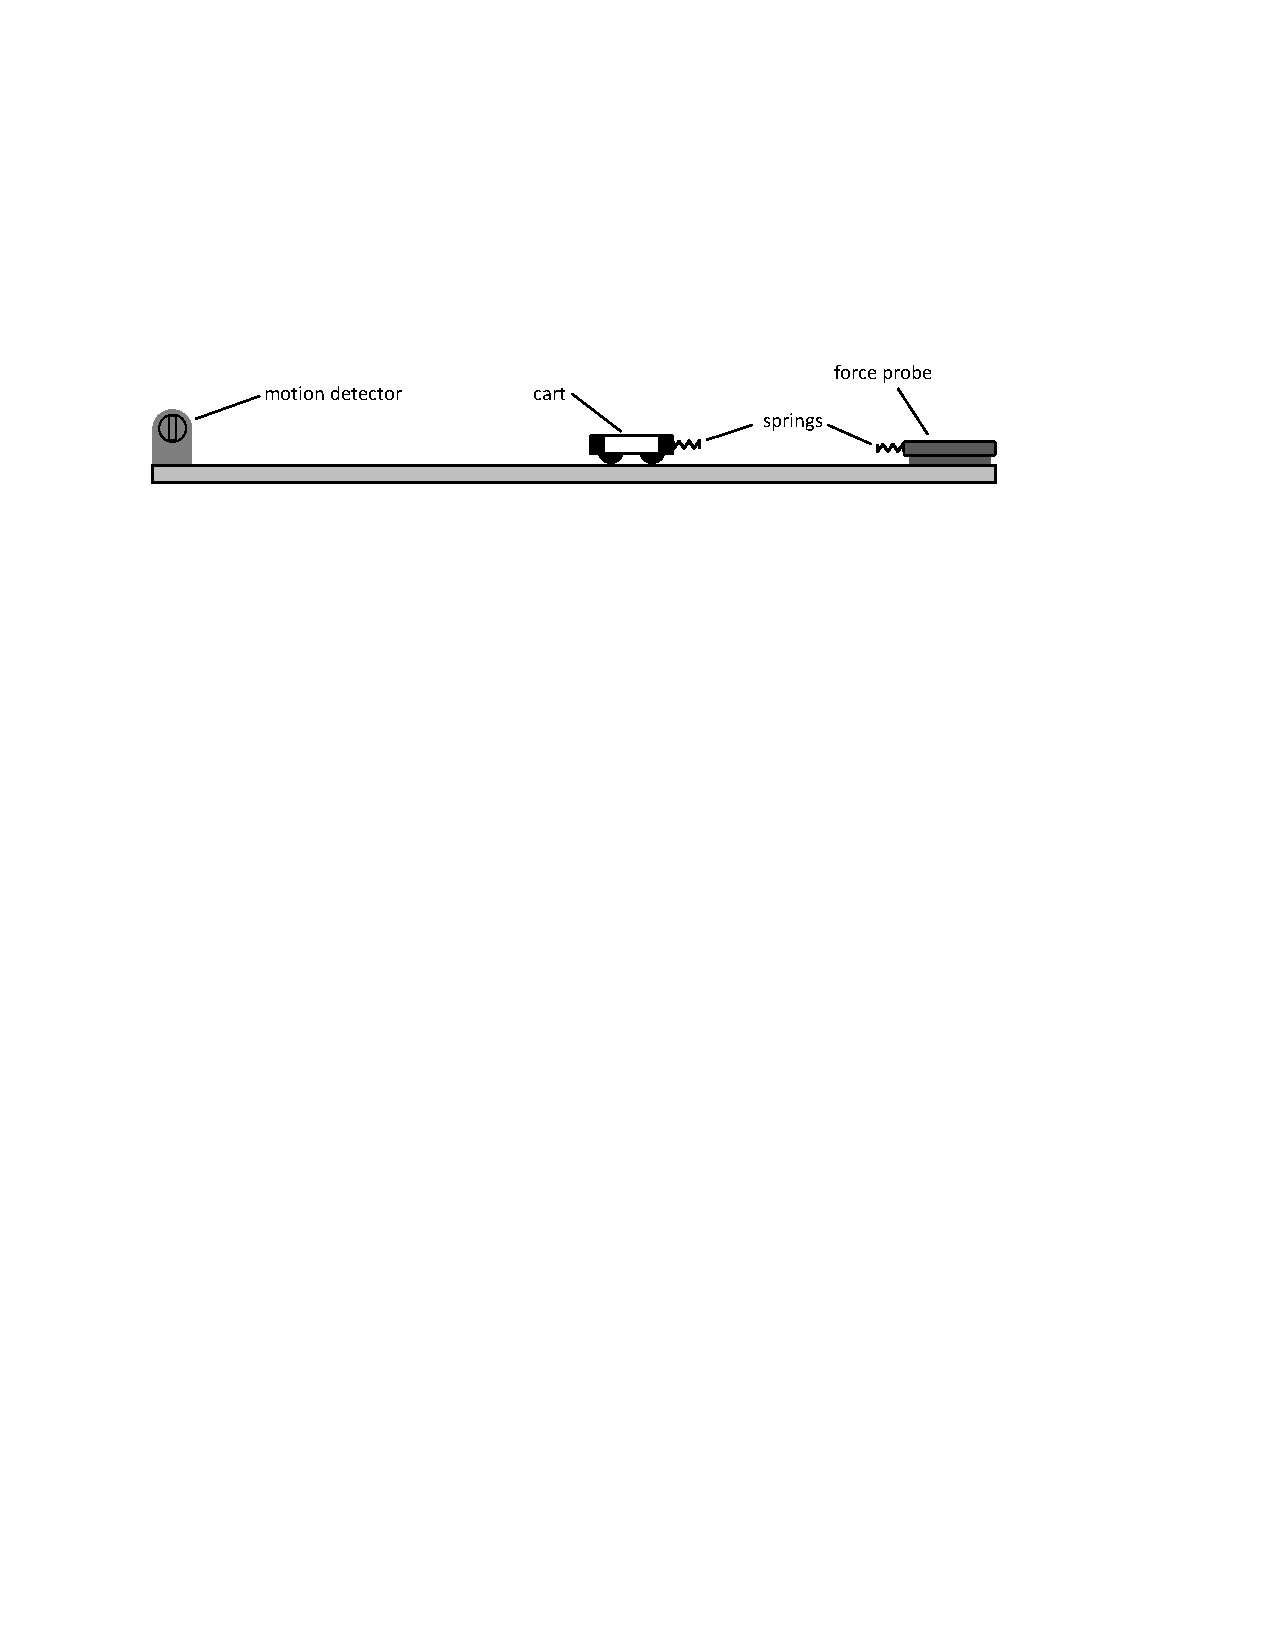
\includegraphics{impulse/cart_ramp_springs.pdf}} %\par}
{\par\centering \resizebox*{0.9\textwidth}{!}{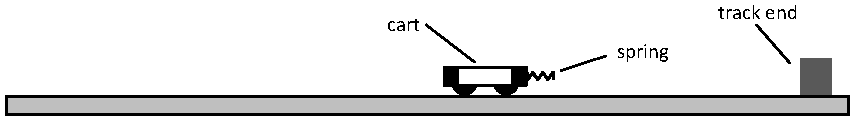
\includegraphics{impulse/cart_spring_collision.pdf}} \par}
\vspace{0.3cm}

(a) Measure the mass $m$ of the cart + spring, using the compact scale, and record it here:
\answerspace{10mm}

(b) With the track horizontal, give the cart a gentle shove towards the track end. The spring attached to the cart's built-in force sensor will measure the force as a function of time during the cart's collision with the track end. Record data in the table below for several trials, using the initial and final velocities of the cart to calculate its change in momentum $\Delta p$.  To calculate the impulse, ${\vec  J}$, you will measure the area under the force curve.  (See \textbf{Appendix \ref{capstone}: Capstone} for instructions on how to measure the area.)

If your instructor requests it, print the graphs for one of your trials and include it with this report.  Also, you can use {\it Excel} to make your table instead if you prefer, but be sure to print it and attach it at the end of this unit. 

\begin{center}
{\renewcommand{\arraystretch}{2.0}
\begin{tabular}{|c|c|c|C{0.8in}|c|C{1in}|} \hline 
$v_i$ (m/s) & $v_f$ (m/s) & $\Delta p$ (kg$\cdot$m/s) & $J$ (N$\cdot$s) & difference & \% difference \\ 
\hhline{|=|=|=|=|=|=|}
& & & & & \\ \hline 
& & & & & \\ \hline 
& & & & & \\ \hline 
& & & & & \\ \hline 
& & & & & \\ \hline 
& & & & & \\ \hline 
\end{tabular} }
\end{center}

(c) For each trial above, calculate the difference between $J$ and $\Delta p$, expressing it as a percentage difference as well.  


(d) Do your results verify the impulse-momentum theorem? Explain, \textit{quantitatively}.
\answerspace{1in}


\pagebreak
(e) What do you expect for the values in the last column of your table (Percent diff)? Make a histogram of your results in the \% difference column and calculate the average and standard deviation. For information on making histograms, see \textbf{Appendix \ref{excel}}. For information on calculating the average and standard deviation, see \textbf{Appendix \ref{treatment}} (can also be done in \textit{Excel}). Record the average and standard 
deviation here. Attach the histogram to this unit. Is your data consistent with your expectation?
\answerspace{25mm}

(f) What does the histogram of your data tell you?
\answerspace{25mm}

(g) Is there any indication of a systematic uncertainty? What are the possible
sources of error?
\answerspace{25mm}
